\chapter{Model} \label{sec:model}


\section{Problem derivation}

To define the problem, we start with the Maxwell equations and corresponding constitutive relations. The Maxwell equations are given by
\begin{align*}
    \nabla \times \mathbf{E} &= -\frac{\partial \mathbf{B}}{\partial t}, \\
    \nabla \times \mathbf{H} &=  \mathbf{J} + \frac{\partial \mathbf{D}}{\partial t}, \\
    \nabla \cdot \mathbf{B} &= 0, \\
    \nabla \cdot \mathbf{D} &= \rho,
\end{align*}
where
\begin{itemize}
    \item $\mathbf{E}, [V/m]$ is the electric field intensity,
    \item $\mathbf{H}, [A/m]$ is the magnetic field intensity,
    \item $\mathbf{J}, [A/m^2]$ is the current density,
    \item $\mathbf{B}, [T]$ is the magnetic flux density,
    \item $\mathbf{D}, [C/m^2]$ is the electric flux density,
    \item $\rho, [C/m^3]$ is the free charge density.
\end{itemize}

\noindent These have the following constitutive relations:
\begin{align*}
    \mathbf{J} &= \mathbf{J_e} + \mathbf{J_c} \\
    \mathbf{B} &= \mu\mathbf{H} \\
    \mathbf{J}_c &= \sigma\mathbf E \\
    \mathbf{D} &= \epsilon \mathbf E
\end{align*}
where
\begin{itemize}
    \item $\mathbf{J_e}$ is the external current density,
    \item $\mathbf{J_c}$ is the conduction current density,
    \item $\sigma$ is the conductivity of the material,
    \item $\mu = \mu_0\mu_r$ is the permeability of the core,
    \item $\epsilon = \epsilon_0\epsilon_r$ is the permittivity of the material.
\end{itemize}

\begin{assumption}
    The permittivity of vacuum $\epsilon_0$ is very small, $(\mathcal{O}(10^{-12}))$, and for all materials in this research $\epsilon_r < 10$, so $\epsilon$ can be neclegted. Therefore, $\mathbf{D} \approx 0$ and can be neglected.
\end{assumption}

\noindent Substituting this in the Maxwell equations yields three equations,
\begin{align*}
    \nabla \times \mathbf{E} &= -\frac{\partial \mathbf{B}}{\partial t}, \\
    \nabla \times \left[\mu^{-1}\mathbf{B}\right] &=  \mathbf{J_e} + \sigma \mathbf{E}, \\
    \nabla \cdot \mathbf{B} &= 0.
\end{align*}

\noindent Using the potential formulation,
\begin{align*}
    \mathbf{E} &= -\nabla \varphi -\frac{\partial \mathbf{A}}{\partial t}, \\
    \mathbf{B} &= \nabla \times \mathbf A,
\end{align*}
we can formulate a system that we can solve.

\begin{assumption}
    We assume that the contribution of the electrostatic field $\varphi$ is negligble compared to the contribution of the potential field $\mathbf A$. That is, $\nabla \varphi = 0$, which implies that $\mathbf{E} = -\frac{\partial \mathbf{A}}{\partial t}$.
\end{assumption}

\begin{assumption}
    The flow of current is oriented along the $z$ axis, and the geometry is in the $xy$ plane. That is, $\mathbf{A} = (0, 0, A_z)$ and $\mathbf{J_e} = (0, 0, J_z)$. This implies $\nabla \times \mathbf A = (\partial_y A_z, -\partial_x A_z,0)$.
\end{assumption}

\noindent Substituting these assumptions into the Maxwell equations and rearranging, we obtain our problem definition.
\begin{equation*}
    \sigma\frac{\partial A_z}{\partial t} = - \left(\frac{\partial}{\partial x}\left[\frac{1}{\mu} \frac{\partial A_z}{\partial x}\right] + \frac{\partial}{\partial y}\left[\frac{1}{\mu} \frac{\partial A_z}{\partial y}\right]\right) + J_z,
\end{equation*}

\begin{problem}
    Find $A_z$ in the system
    \begin{equation}
        \sigma\frac{\partial A_z}{\partial t} = - \nabla \cdot \left(\frac{1}{\mu} \nabla A_z \right) + J_z,
    \end{equation}
    where
    \begin{itemize}
        \item $A_z$ is the magnetic vector potential in the $z$ direction,
        \item $\mu$ is the permeability of the core,
        \item $J_z$ is the imposed source current density,
        \item $\sigma$ is the conductivity of the core.
    \end{itemize}
    From this point onwards, this will be formulated as
    \begin{equation}
        \sigma\dot u = \nabla \cdot \left[\frac{1}{\mu}\nabla u\right] + f.
    \end{equation}
\end{problem}

\newpage
\section{Spatial discretisation using finite element method}

\begin{figure}
    \centering
    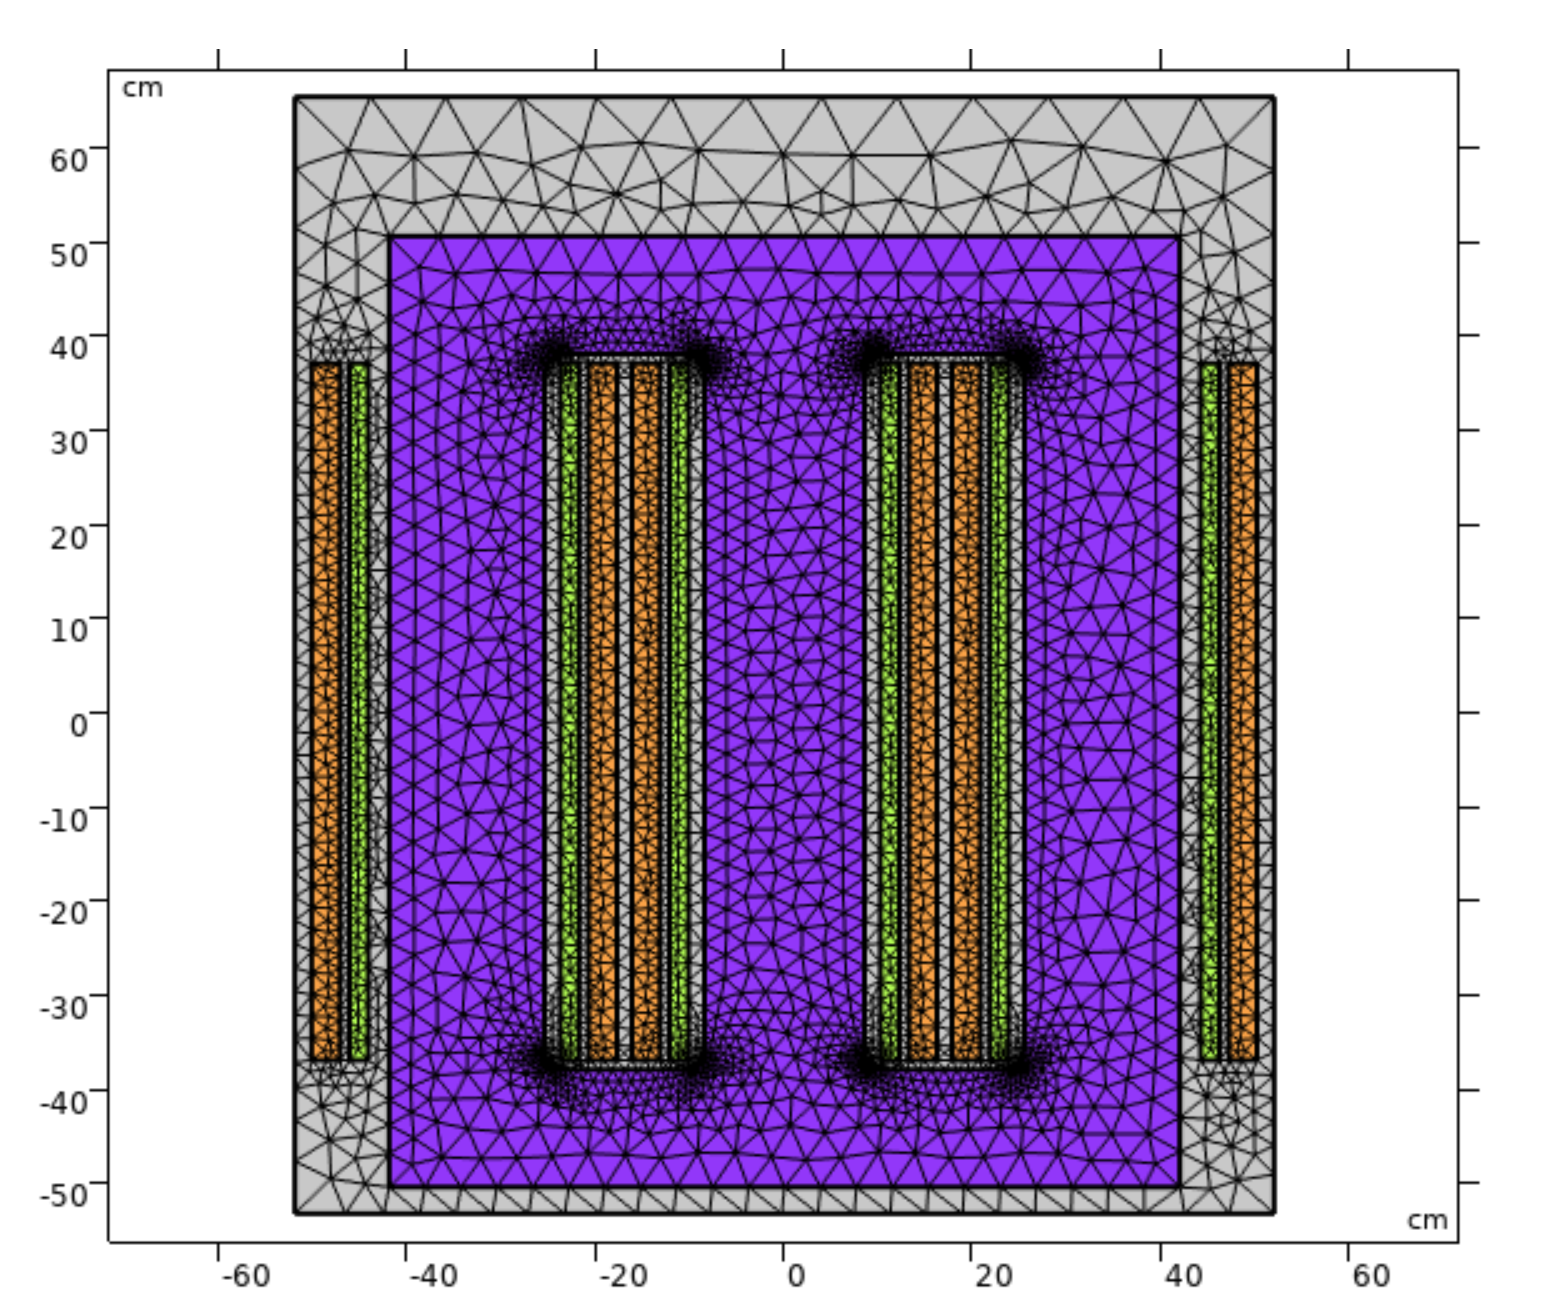
\includegraphics[width=0.5\textwidth]{img/regular_mesh.png}
    \caption{The mesh used to discretize the domain (\cite{vanDijk2022}).}
    \label{fig:regular_mesh}
\end{figure}

To solve this system, the finite element method can be used. Choosing a first order basis function 
\[
    \phi_i = a_i + b_i x + c_i y,
\]
for each node $i$, the solution $u$ can be approximated as
\[
    u = \sum_{i=1}^N u_i \phi_i.
\]
This results in the following weak form.
\begin{weakform}
    \begin{equation}
        \sigma M \dot u = K(\mu(u)) u + f,
        \label{eqn:weakform}
    \end{equation}
    where
    \begin{itemize}
        \item $u$ is $A_z$, the solution.
        \item $M$ is the mass matrix,
        \item $K$ is the stiffness matrix,
        \item $f$ is the source term, given by $J_z$,
    \end{itemize}
\end{weakform}

\noindent The mass matrix on element $e_k$,  $M_{e_k}$ is given by
\begin{align*}
    M_{e_k} = \left[\int_{\Omega_{e_k}}\phi_i\phi_j d\Omega \right]_{1 \leq i, j \leq 3}
\end{align*}

\noindent Similarly, the local stiffness matrix $K_{e_k}$ is given by
\begin{align*}
    K_{e_k}(\mu(u)) &= \left[\int_{\Omega_{e_k}} \phi_i \nabla \cdot \left(\frac{1}{\mu} \nabla \cdot \phi_j \right) d \Omega \right]_{1 \leq i, j \leq 3} \\
    &= -\int_{\Omega_{e_k}} \frac{1}{\mu} \nabla \phi_i \nabla \phi_j d \Omega
\end{align*}

\noindent Similarly the local source term $f_{e_k}$ is given by
\begin{align*}
    f_{e_k}(t) = \left[\int_{\Omega_e} f(x,y,t) \phi_i d \Omega\right]_{1 \leq i \leq 3}\\
\end{align*}

\noindent We can exactly calculate the integrals using the following quadrature rule for first order polynomials.
\begin{align*}
    \int_{\Omega_e}g(x,y)dxdy = A_{e_k}\bar{g}_{e_k}, \\
\end{align*}
where $A_{e_k}$ is the area of element $e_k$ and $\bar{g}_{e_k}$ is the average of function $g$ over element $e_k$.

\subsection{Time dependence}
If $\mu$ is constant we may write $K(\mu(u)) = K(\mu) = \frac{1}{\mu}K$. In this case the use of separation of variables is valid. 
If $\mu$ is dependent on $u$, separation of variables is not valid due to the non-linear nature of the problem. 
In this case a time stepping method is necessary. This section outlines both approaches and their implementation.
Ultimately, the time stepping method is used, because the permeability this paper is concerned with the non-linear case.

\subsection{Separation of variables}
Applying separation of variables
\begin{align*}
    u(x,y,t) = \hat u(x,y) \cdot e^{j\omega t}.
\end{align*}
to the weak form \eqref{eqn:weakform} yields
\begin{equation*}
    \left[\sigma \omega j M + \frac{1}{\mathbf \mu}A\right]\hat u = \hat f.
\end{equation*}
This is a linear system of equations, which can be solved using a linear solver. 
Additionally it may be solved for multiple frequencies $\omega_1, \omega_2, \dots$ by writing
\begin{equation}
    u(x,y,t) = \hat u_1(x,y) e^{j\omega_1 t} + \hat u_2(x,y) e^{j\omega_2 t} + \dots,
\end{equation}
solving the above system for each frequency, and summing the solutions. However it must be noted that the influence of the frequencies on each other is not taken into account in this approach.
This is why the time stepping method is used in this paper.

\subsection{Time stepping}
The time derivative in equation \ref{eqn:weakform} can be approximated using a backward Euler method, 
\begin{equation*}
    \sigma M\frac{u^{k} - u^{k-1}}{\Delta t} = K(u^{k}) u^{k} + f^{k},
\end{equation*}
where $u^k$ is the solution at time $t^k$ and $u^{k+1}$ is the solution at time $t^{k+1} = t^k + \Delta t$.
This leads to the following implicit time stepping scheme.
\begin{equation*}
    \left[\sigma M - \Delta t K(u^{k-1})\right]u^{k} = \sigma M u^{k-1} + \Delta t f^{k}.
\end{equation*}
During each time step, this non-linear system of equations must be solved. This is done using an iterative scheme with dampening factor $\alpha$. This means that instead of $u^k_i$, there is $\tilde{u}^k_i$, defined by
\begin{equation*}
    \tilde{u}^k_{i} = \alpha \tilde{u}^k_{i-1} + (1-\alpha)u^k_{i-1},
\end{equation*}
where the superscript $k$ denotes time, and subscript $i$ denotes the iteration number. This is then used for solving the system of equations for $u^k_i$:
\begin{equation}
    \left[\sigma M - \Delta t K(\tilde{u}^k_{i})\right] u^k_{i} = \left[\sigma M \tilde{u}_{i}^{k} + \Delta t f^{k}\right].
\end{equation}

\noindent This is repeated until the residual is sufficiently small. That is
\begin{equation*}
    ||u^k_{i-1} - u^{k}_i||_2 \leq \epsilon,
\end{equation*}
where $\epsilon$ is a small number. In this paper $\epsilon = 10^{-3}$ is used. The full algorithm is given in Algorithm \ref{alg:time_stepping}.


\begin{algorithm}
    \caption{\label{alg:time_stepping} Time-stepping algorithm using Backward Euler}
    \begin{algorithmic}[1]
    \Function{nonlinear-solve}{}
    \State $u^0 \leftarrow \textbf{0}$
    \For{$k \in [0, N_t]$}{}
        \State $i \leftarrow 0$
        \State $u^k_0 \leftarrow u^{k-1}$
        \State $\tilde{u}^k_0 \leftarrow u^{k-1}$
        \While{$\Delta u \leq \epsilon$}{}
            \State $i \leftarrow i + 1$
            \State $\tilde{u}^k_{i} \leftarrow \alpha \tilde{u}^k_{i-1} + (1-\alpha)u^k_{i-1}$
            \State $u^k_{i} \leftarrow \left[\sigma M - \Delta t K(\tilde{u}^k_{i})\right]^{-1}\left[\sigma M \tilde{u}_{i}^{k} + \Delta t f^{k}\right]$
            \State $\Delta u \leftarrow ||u^k_{i-1} - u^{k}_i||_2$
        \EndWhile
        \State $u^{k+1} \leftarrow u^k_i$
    \EndFor
    \EndFunction
    \end{algorithmic}
\end{algorithm}